%  NOTE: Please make sure to completely fill out the \def parts in meta-data.tex!

\section*{Preface}
Some room for acknowledgements.

\newpage \thispagestyle{empty} \strut
\newpage \pagenumbering{arabic}

\title{\thesistitle{}}
\author{\yourname}

\maketitle % Yes, again

\begin{abstract}

\end{abstract}

\section{Introduction}

early linguistics vs early sign language study



\section{Related Work}

Stokoe, W., Jr.
1960. Sign Language Structure: An Outline of the Visual Communication
Systems of the American Deaf. (Studies in linguistics: occasional papers
8) Buffalo, NY: University of Buffalo. [Rev. edn., Silver Spring, MD: Linstok
Press, 1978].
sign language us actually a language

\section{Experimental Setup}



\subsection{Data}

\subsubsection{Source}

The data consists of $405$ EAF-files (ELAN Annotation Files) gathered by the Institute for German Sign Language and Communication of the Deaf at Hamburg University \cite{prillwitz2008dgs}. These files consist of a total of $50$ hours of annotated recordings spanning a wide range of narrations regarding the cultural aspects of the deaf community. The interviews were conducted using a peer-to-peer procedure, where participant change roles according to the conversation \cite{prillwitz2008dgs}. During a discussion $2$ German Sign Language or Deutsche Gebärdensprache (DGS) signers conversed. Each conversation consisted of a standardized interview covering linguistical and social data \cite{deaf_areas}. Following this conversation, a spontaneous conversation on a given topic was held while the participants were encouraged to use as much basic vocabulary as possible \cite{deaf_areas}. In the EAF-files the signers are annotated as either Speaker A or Speaker B. The data was collected between January $2010$ and December $2011$  by videotaping $330$ participants from all $16$ Federated States (Bundesländer). The recordings were conducted using a mobile field lab in:

\begin{itemize}
  \item Areas with a relatively high deaf population density (deaf schools, deaf centres, and deaf institutes). \cite{age_data_hamburg} \cite{deaf_areas}
  \item The catchment areas of the former Schools for the Deaf.\cite{age_data_hamburg} \cite{prillwitz2008dgs}
  \item Areas which were easy to reach from surrounding rural communities. \cite{age_data_hamburg} \cite{deaf_areas}
  \item Areas that were suspected of having a distinct dialect. \cite{age_data_hamburg} \cite{prillwitz2008dgs}
\end{itemize}

 The data was collected by representatives of the local deaf community to take into account the regional varieties of DGS \cite{deaf_areas}. As can be seen in \autoref{fig:bundeslander} the data was sampled from participants across different age groups \cite{age_data_hamburg}. 


% Age category figure
\pgfplotstableread[row sep=\\,col sep=&]{
    interval & carT & carD \\
    18--30     & 12.1  & 12.4  \\
    31--45     & 13.6 & 13.9  \\
    46--60   & 12.7 & 12.4 \\
    61+   & 11.5 & 11.2 \\
    }\mydata

\begin{figure}[h]
\begin{tikzpicture}
    \begin{axis}[
            ybar,
            bar width=.6cm,
            width=.8\textwidth,
            height=.5\textwidth,
            legend style={at={(0.5,1)},
                anchor=north,legend columns=-1},
            symbolic x coords={18--30,31--45,46--60,61+},
            xtick=data,
            nodes near coords,
            nodes near coords align={vertical},
            ymin=0,ymax=25,
            xlabel={\/Age categories},
            ylabel={\/Percentage of participants (\%)},
        ]
        \addplot table[x=interval,y=carT]{\mydata};
        \addplot table[x=interval,y=carD]{\mydata};
        \legend{Male, Female}
    \end{axis}
    
\end{tikzpicture}
\caption{Showing the percentage of participants per age , divided into both the Male (shown in Purple) and Female (shown in Red) gender,  that participated in the creation of the DGS corpus (both annotated and non-annotated). \cite{age_data_hamburg}}
\label{fig:bundeslander}
\end{figure}

\subsubsection{ELAN}
The conversation conducted between the representatives of the deaf community has been annotated and stored in EAF-files. These EAF-files can be shown and edited using the ELAN software \cite{crasborn2008enhanced}. ELAN is a multimedia annotation software developed by \citep{elan_software} to assist in Linguistical studies, language conservation, and sign language research \cite{brugman2004annotating}. The software can be used to add annotations to video and/or audio recordings. An annotation can be a sentence, word, or in the case of sign language, a gloss. Using ELAN multiple annotations can be created that are sorted into tiers \cite{crasborn2008enhanced}.  

% EAF-example
\begin{figure}[h]
 \centering 
 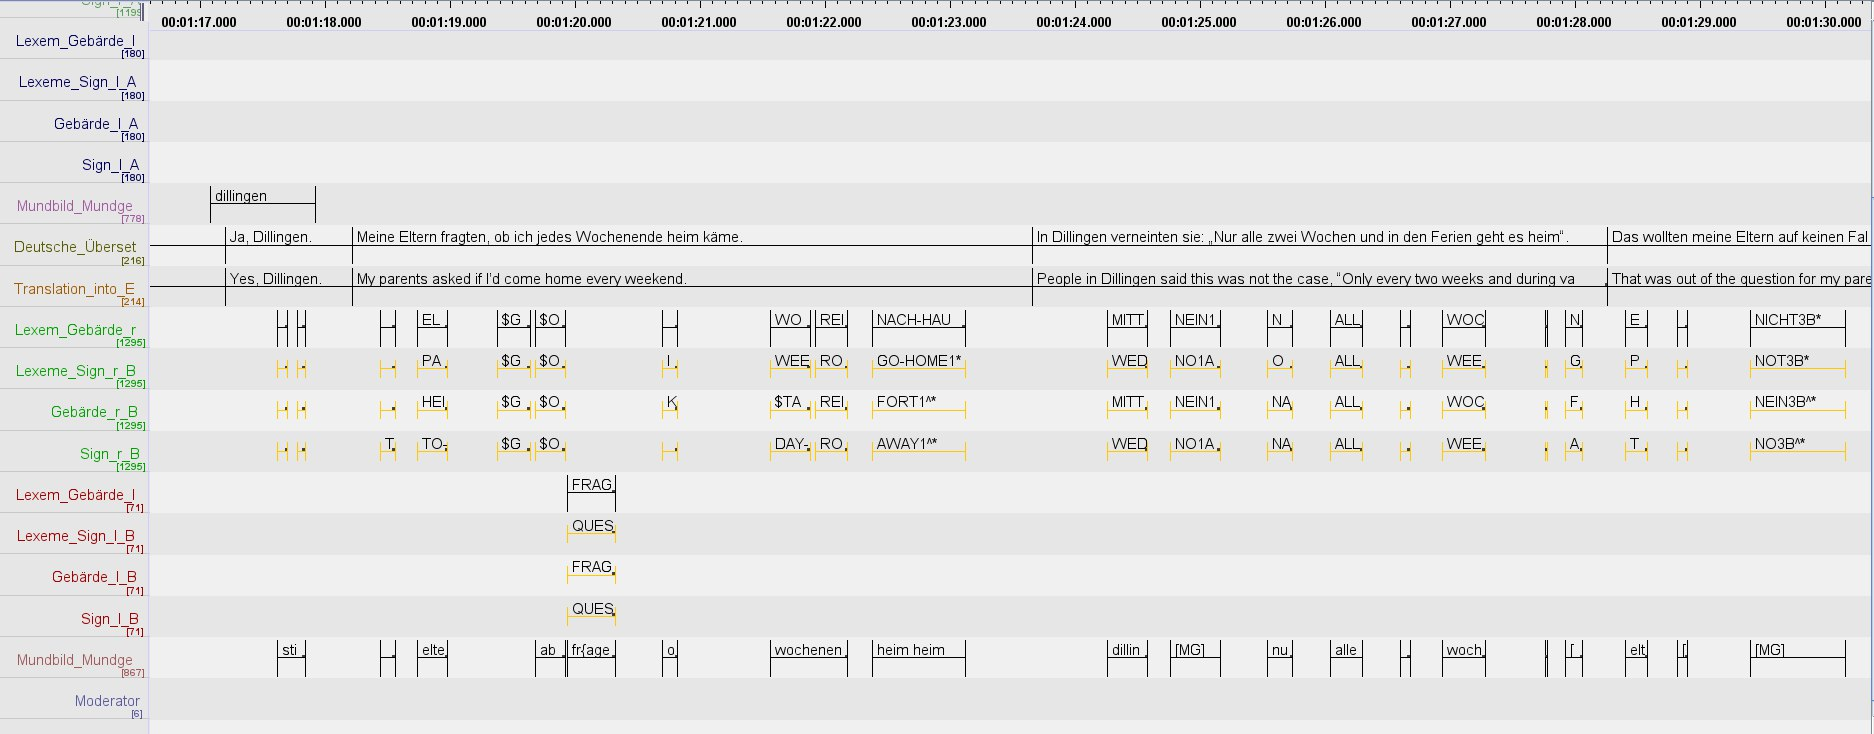
\includegraphics[width=14cm]{Bachelor CSAI thesis template/images/ELAN_example.jpg}
 \caption{Showing the structure of one of the EAF (English Annotated File)-files \cite{elan_example} inside the program ELAN. ELAN is a multimedia annotation tool used for multi-modality research \cite{sloetjes2017elan}. }
 \label{fig:elan_example}
\end{figure}

\subsubsection{Initial Translation}

The annotations divided into tiers are presented across a timeline. As can be seen in \autoref{fig:elan_example}these files are divided into $11$ different tiers, presented in both English and German due to accessibility \cite{konradoffentliches}. Take "Lexem\_Gebärde\_r\_A" for example, this tier is translated into English as "Lexeme\_Sign\_r\_A". The tiers present in the EAF-files, translated into English, are: "Time", "Sign\_l\_B", "Sign\_r\_B", "Lexeme\_Sign\_l\_B", "Lexeme\_Sign\_r\_B", 
"Translation\_into\_English\_B", "Sign\_l\_A", "Sign\_r\_A", "Lexeme\_Sign\_l\_A", "Lexeme\_Sign\_r\_A", and "Translation\_into\_English\_A" \cite{sloetjes2017elan}. The goal of this paper is to, through experimentation, show to what extent temporal data aids in the performance of a machine translation system for sign language glosses to text. For this purpose, both the German Sign Language and the German Language were chosen respectively. Since the target language is German it was decided to use the original glosses and translations that were available in the corpus.

The initial translation of the glosses in the data set (i.e.: Sign\_l\_A to Translation\_into\_English) was conducted by contracted sign language translators and interpreters \cite{konradoffentliches}. These researchers translated the data set word-for-word. Consequently, university students created coherent meaningful sentence like structures. Lastly, these sentences were fed back into the system until the proper meaning was determined by the DGS experts (\autoref{fig:uselesspipeline}) \cite{konradoffentliches}.

\begin{figure}[h]
 \centering 
 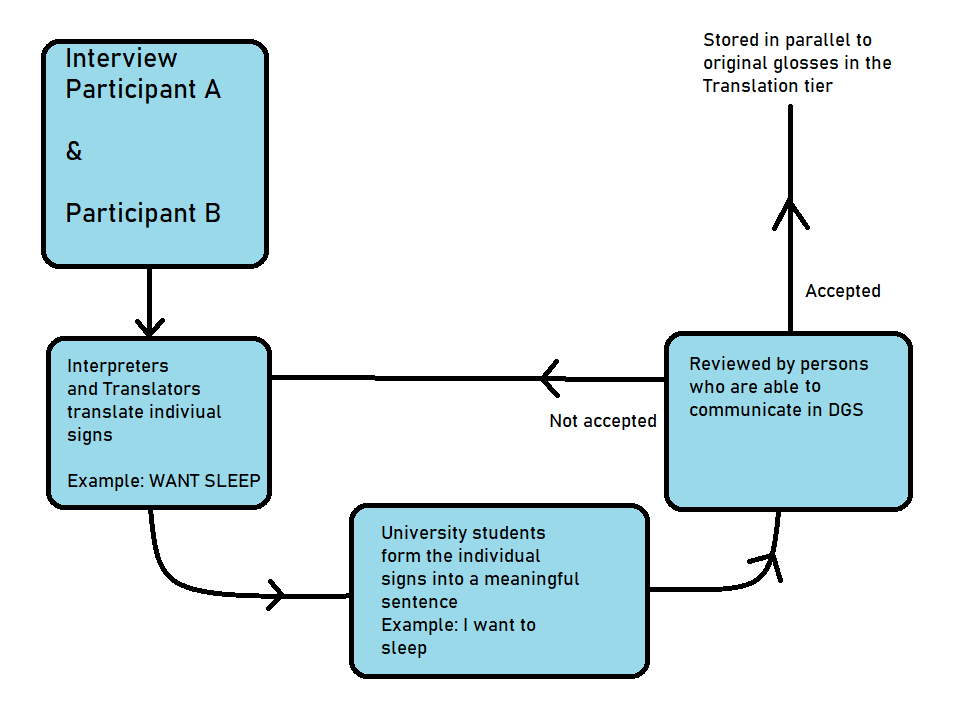
\includegraphics[width=14cm]{Bachelor CSAI thesis template/images/translation_pipeline.png}
 \caption{Showing the translation pipeline of the initial translation phase as conducted by the Institute for German Sign Language and Communication of the Deaf at Hamburg University. \cite{konradoffentliches} }
 \label{fig:uselesspipeline}
\end{figure}

\subsubsection{Segmentation}

As with spoken languages, sign languages tend not to have a naturally occurring white space character \cite{hankesegmentation} \cite{konradoffentliches}. Thus it is difficult to determine where a sign begins and where a sign ends. In this situation, the segmentator has two options: either add a gap or none at all. Unlike spoken languages, when a participant is signing two words, take TREE (rest your right forearm upon your left palm and twist) \cite{perniss2007space} and COW (make two horns using your thumb and little finger on top of your head), for example. There is a transitional period where the participant moves his or her arm from one sign to the next. When adding a gap between the signs, the segmentator determines that the transitional movements are not part of the token's form \cite{konradoffentliches}. Taking this into account researchers at the University of Hamburg have decided that for the creation of the DGS corpus gaps will be added. The direct result of this decision is located in the EAF files, where there is temporal data with no associated annotations.

\subsubsection{Lemmatisation and Gloss conventions}

When creating a corpus there is an intrinsic need to have conventions in place to make sure a uniform dataset is created. \cite{konradoffentliches} Therefore it is necessary to employ linguistics to standardise glosses using gloss conventions: \cite{kristoffersen2016designing}

\begin{itemize}
    \item In the field of Linguistics or more specifically in the field of lexicography, a lexical item forms the basic element of the lexicon of a language. Lexical signs are treated as items, that is as units of their respective sign language that would be found in the dictionary \cite{konradoffentliches}. When a deaf person signs SQUARE1\textasciicircum  it may mean different things such as map, recipe, or page. In DGS \cite{perniss2007space} and several other European Sign Languages signs are iconically motivated \cite{pietrandrea2002iconicity} \cite{oomen2017iconicity}, meaning that there is a similarity between the form of the sign and the meaning of the sign. In the DGS corpus, type glosses are given an indication of iconic value by using a circumflex at the end: "SQUARE1\textasciicircum ". Examples of child types to the SQUARE1\textasciicircum parent type are: FORM1, MIRROR2, and PAPER4, these and all other non-circumflex glosses are sub types. The numbers denote different lexical variants.
    \item Fully iconically motivated signs, also known as poly-morphemic signs, are denoted as productive signs in contrast to lexical signs that denote something instead of meaning. Productive signs therefore have a \$PROD token \cite{konradoffentliches}
    \item Due to the anonymisation laws present in Germany, where this corpus was created, all names are replaced by "\$NAME". Except when it concerns a famous person the \$NAME gloss is followed by the person's name. \cite{konradoffentliches}
    \item Foreign language elements are represented using the INTS token, for example, when signing the English word Germany instead of "Deutschland" it has been written as GERMANY-INST1.\cite{konradoffentliches}
    \item In German Sign Language it is conventional to use a one-handed manual alphabet, for example when spelling out someones name. For these situations the \$ALPHA token is used. Numbers are presented in a similar manner by using \$NUM. \cite{konradoffentliches}  
\end{itemize}

Taking into account these points a uniform corpus was created with annotated signs presented on a timeline. An example of an annotated DGS sentence can be seen in \autoref{fig:sentence_example}.

\begin{figure}[h]
 \centering 
 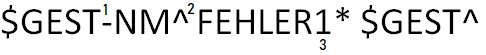
\includegraphics[width=14cm]{Bachelor CSAI thesis template/images/sentence_example.png}
 \caption{Showing an example sentence of the annotated corpus in DGS glosses. The German translation of this gloss sentence is: "Und dann fällt es einem wieder auf, dass der andere noch Fehler macht" \cite{dgscorpus_3}. (English translation: And then one notices again, that the other (person) is still making mistakes). 1. A token denoting a gesture. 2. The sign annotated as NM has iconic meaning. 3. One of several lexical variants of the lexical unit FEHLER. }
 \label{fig:sentence_example}
\end{figure}

\subsubsection{Pre-Processing}
Using the ELAN software $7$ of the $11$ tiers were selected and converted into a CSV file. This creates $2$ distinct CSV files that were consequently merged (\autoref{apx:first}). Due to being able to access the timeline in ELAN, it is possible to extract the temporal features of a given annotation. As mentioned before the  bpe - tokenizing preprocessing


\subsection{Method / Models}

different experiments
opennmt 
-removed white spaces and "nan" to equalize the parallel corpi
-bpe

features in translation
bpe
sentencepiece



\section{Results}

\begin{table}
    
    \label{tab:results}
    \begin{tabular}{llrr}
        \toprule
                                                                  
        Word-Form                   &  Models                           &  BLEU                & TER    \\ 
        \midrule
        \multirow{3}{*}{Original}  &  Baseline                              &   \textbf{3.69}      &  \textbf{0.960} \\
                              & Temporal                                &   2.85               &  0.971 \\
                              & Vocal                                   &   2.03               &  1.000 \\
                              & Combined (Temporal + Vocal)             &   1.69               &  0.973 \\
    
        
    \end{tabular}
    \caption{SCHRIJF HIER NOG IETS}
\end{table}


\section{Discussion}

gebarentaal dialect neit meegomen

schrijf een stuk over wat er gebeurt als je dat hele ding standardised

\section{Conclusion}


\newpage
\bibliography{mybib}

\newpage
\appendix

\appendixsection{Merging Code} \label{apx:first}
\begin{lstlisting}[language=Python, caption=Section 6. Show is the Python code to merge the multiple CSV-files into one DataFrame.]
class create_file(object):
    def __init__(self, path="datasets/"):
        self.path = path
        self.inputs = listdir(str(path))
        self.dataframe = self.drop_empty()

    def clean_dataframe(self, dataset):
        """
        Load the dataset into a frame, delete the "Unnamed" column,
        and replace all instances of nothing with a numpy nan.
        Requires the numpy library.

        :param dataset: str, input name of the dataset.csv
        :return: dataframe, a cleaned dataframe with only used columns
        """
        dataframe = pd.read_csv(self.path + str(dataset), sep=",")  # Read into a frame
        dataframe = dataframe.loc[:, ~dataframe.columns.str.contains("^Unnamed")]  # Drop the "^Unnamed" column
        dataframe.replace("", np.nan, inplace=True)  # Replace the empty values with a nan

        return dataframe

    def merge(self):
        """
        The EAF-files consist of different persons, this functions merges those
        into one dataframe.

        :return: Dataframe. A merged dataframe consisting of all users.
        """
        combined = pd.DataFrame()
        for dataset in self.inputs:
            temp = self.clean_dataframe(dataset)

            # Normalize the column names into the translated versions.
            column_list = list(temp.columns)
            normalized_names = ["Time", "Right", "Mouth", "Translation", "Left"]
            # A dictionary is created with the corresponding column_list name and the normalized name
            translation_dict = {column_list[n]: normalized_names[n] for n in range(len(normalized_names))}
            temp = temp.rename(columns=translation_dict)

            # Combine the dataframes into one universal dataframe
            combined = combined.append(temp, ignore_index=True, sort=False)

        return combined

    def list_definer(self, input_list):
        """
        Finds the True instances in a list and stores their indexes.

        :param input_list: list, a list of True's and False's.
        :return: list, the list of indexes that were true in the input_list.
        """
        output_list = []
        # Looping over a enumerated input_list
        for number, element in enumerate(input_list):
            # If the element is True append the index else continue the loop
            if element:
                output_list.append(number)
            continue
        return output_list

    def drop_empty(self):
        """
        Dropping the empty rows from the dataset causing it to become more information packed.
        Downsides of this approach can be found in the Discussion of the written Thesis.

        :return: dataframe, a dataframe where there are no empty rows.
        """
        combined = self.merge()

        # Find the empty rows for each respective token (time excluded since it is always present).
        left_sign = set(self.list_definer(list(combined['Left'].isnull().values)))
        right_sign = set(self.list_definer(list(combined['Right'].isnull().values)))
        mouth_token = set(self.list_definer(list(combined['Mouth'].isnull().values)))

        # Find the intersection of these tokens.
        signs = left_sign.intersection(right_sign)
        empty_rows = signs.intersection(mouth_token)
        signs_missing = list(empty_rows)

        # Dropping the empty rows
        final_dataframe = combined.drop(signs_missing)

        return final_dataframe
\end{lstlisting}
 

